% !TEX root = ../main.tex

\section{Results and discussion}

A sensitivity analysis of the pyrolysis kinetics in a batch reactor model are discussed in this section. Biomass composition and batch reactor model results for the Blend3 feedstock are also explored.

\subsection{Pyrolysis kinetics sensitivity analysis}

A sensitivity analysis of the Debiagi pyrolysis kinetics in a batch reactor model was performed using 16,000 samples which represent a range of biomass compositions. A reaction time of 10 seconds, a reactor temperature of 773.15 K, and a reactor pressure of 101,325 Pa were applied to the model. Batch reactor yields from the samples are shown in Figures \ref{fig:batch-sa1} and \ref{fig:batch-sa2}. The most pronounced gas trends are observed for the lignin-o, tannin, and triglyceride concentrations while liquids appear to be most affected by triglycerides. The greatest affects on solid yields seem to be from tannin and triglyceride concentrations.

The Sobol sensitivity analysis based on the batch reactor results is presented in Figure \ref{fig:batch-sa3}. The results from the first-order indices (S1) are discussed below. Similar results are observed for the total-order indices (ST).

\begin{itemize}
    \item gas yields are most affected by lignin-o, tannins, and triglycerides
    \item liquid yields are most affected by triglycerides and to a lesser extent by tannins and cellulose
    \item solid yields are most affected by cellulose, tannins, and triglycerides
\end{itemize}

\begin{figure}[H]
    \centering
    \makebox[\textwidth][c]{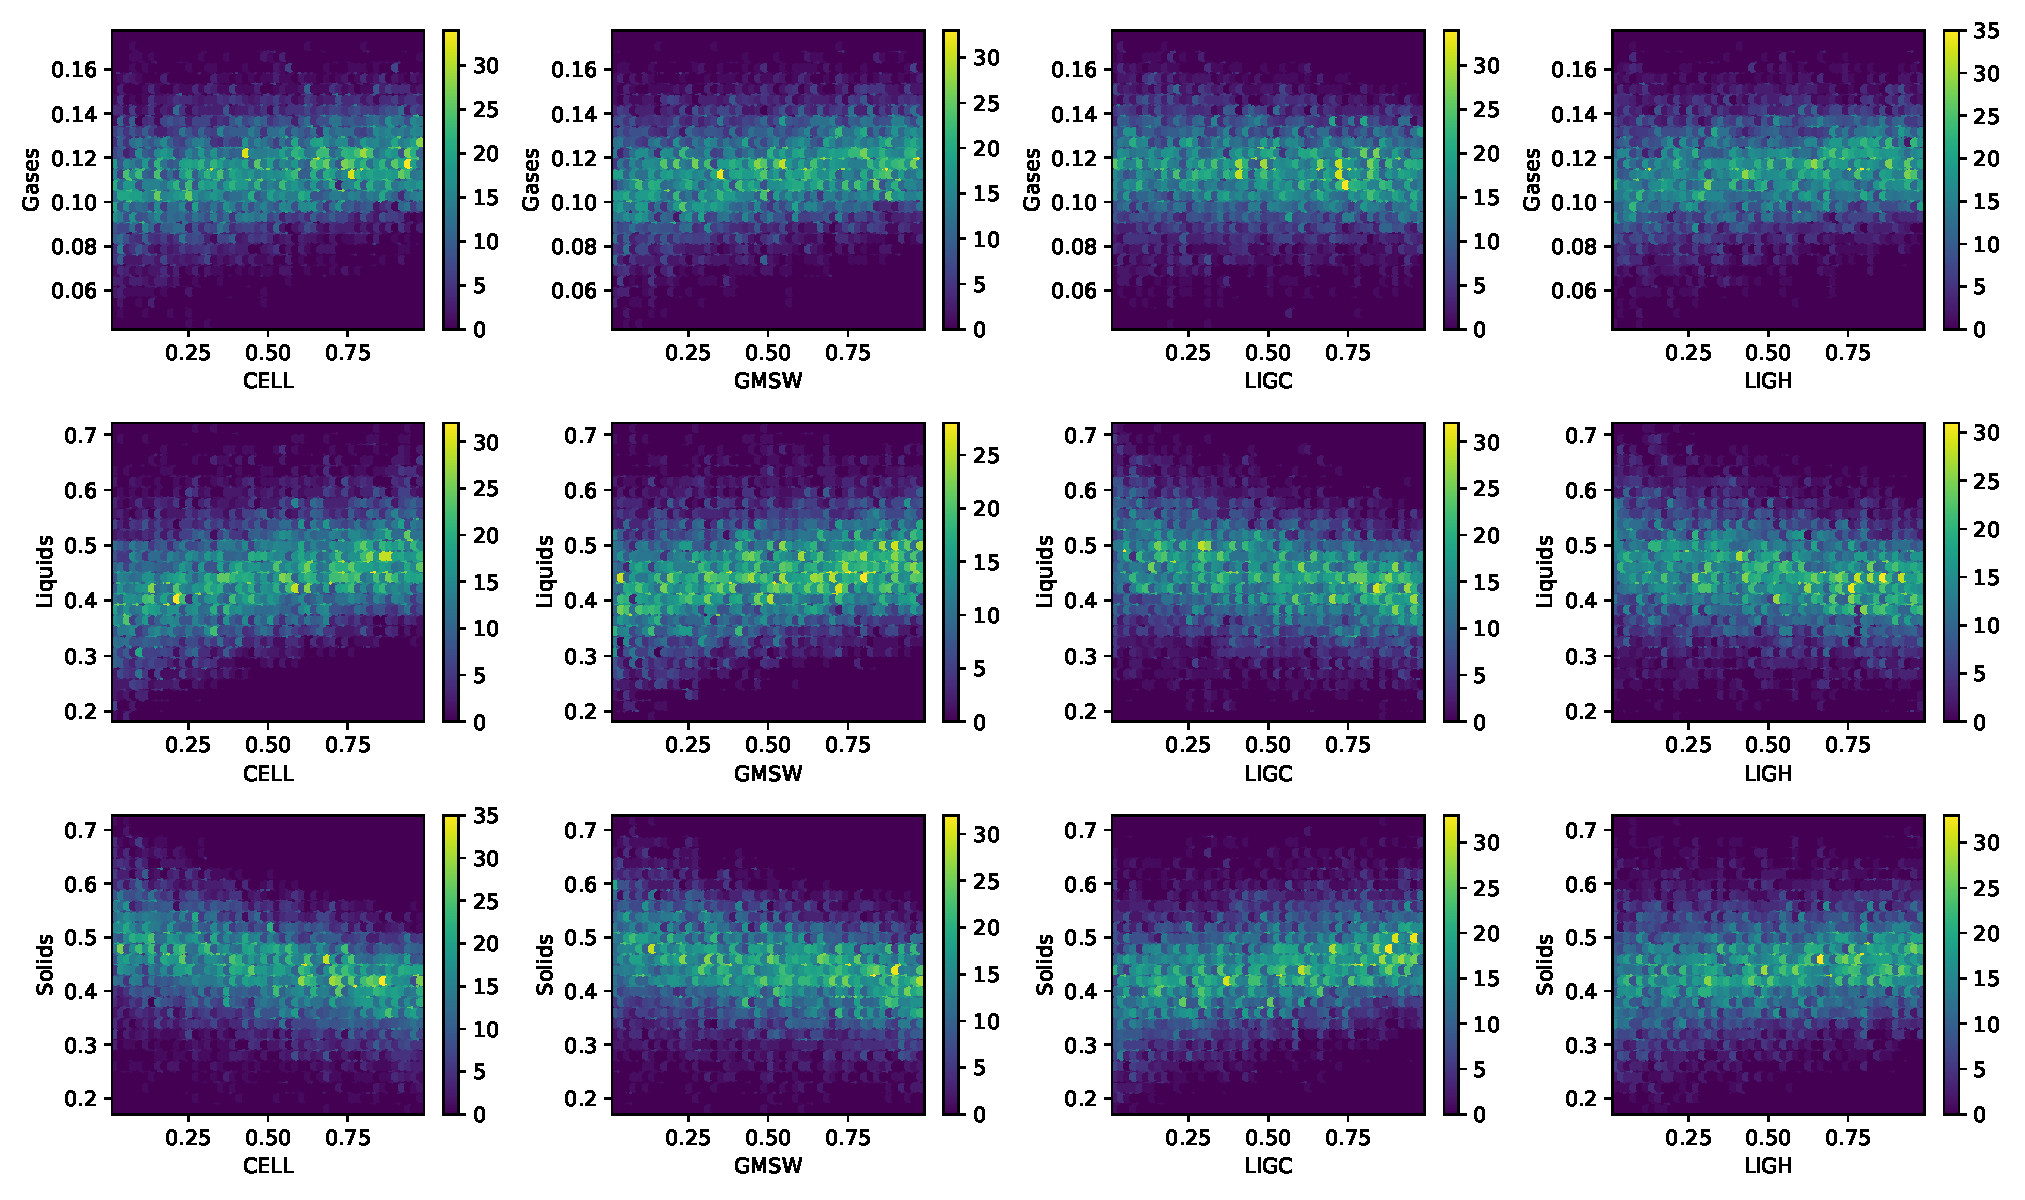
\includegraphics[width=1.3\textwidth]{figures/sa-hexbin1-n1000.pdf}}
    \caption{Batch reactor results for cellulose, hemicellulose (GMSW), carbon-rich lignin (LIGC), and hydrogen-rich lignin (LIGH) using 16,000 samples. Reaction time is 10 seconds at 773.15 K and 101,325 Pa. Colorbar represents bin count.}
    \label{fig:batch-sa1}
\end{figure}

\begin{figure}[H]
    \centering
    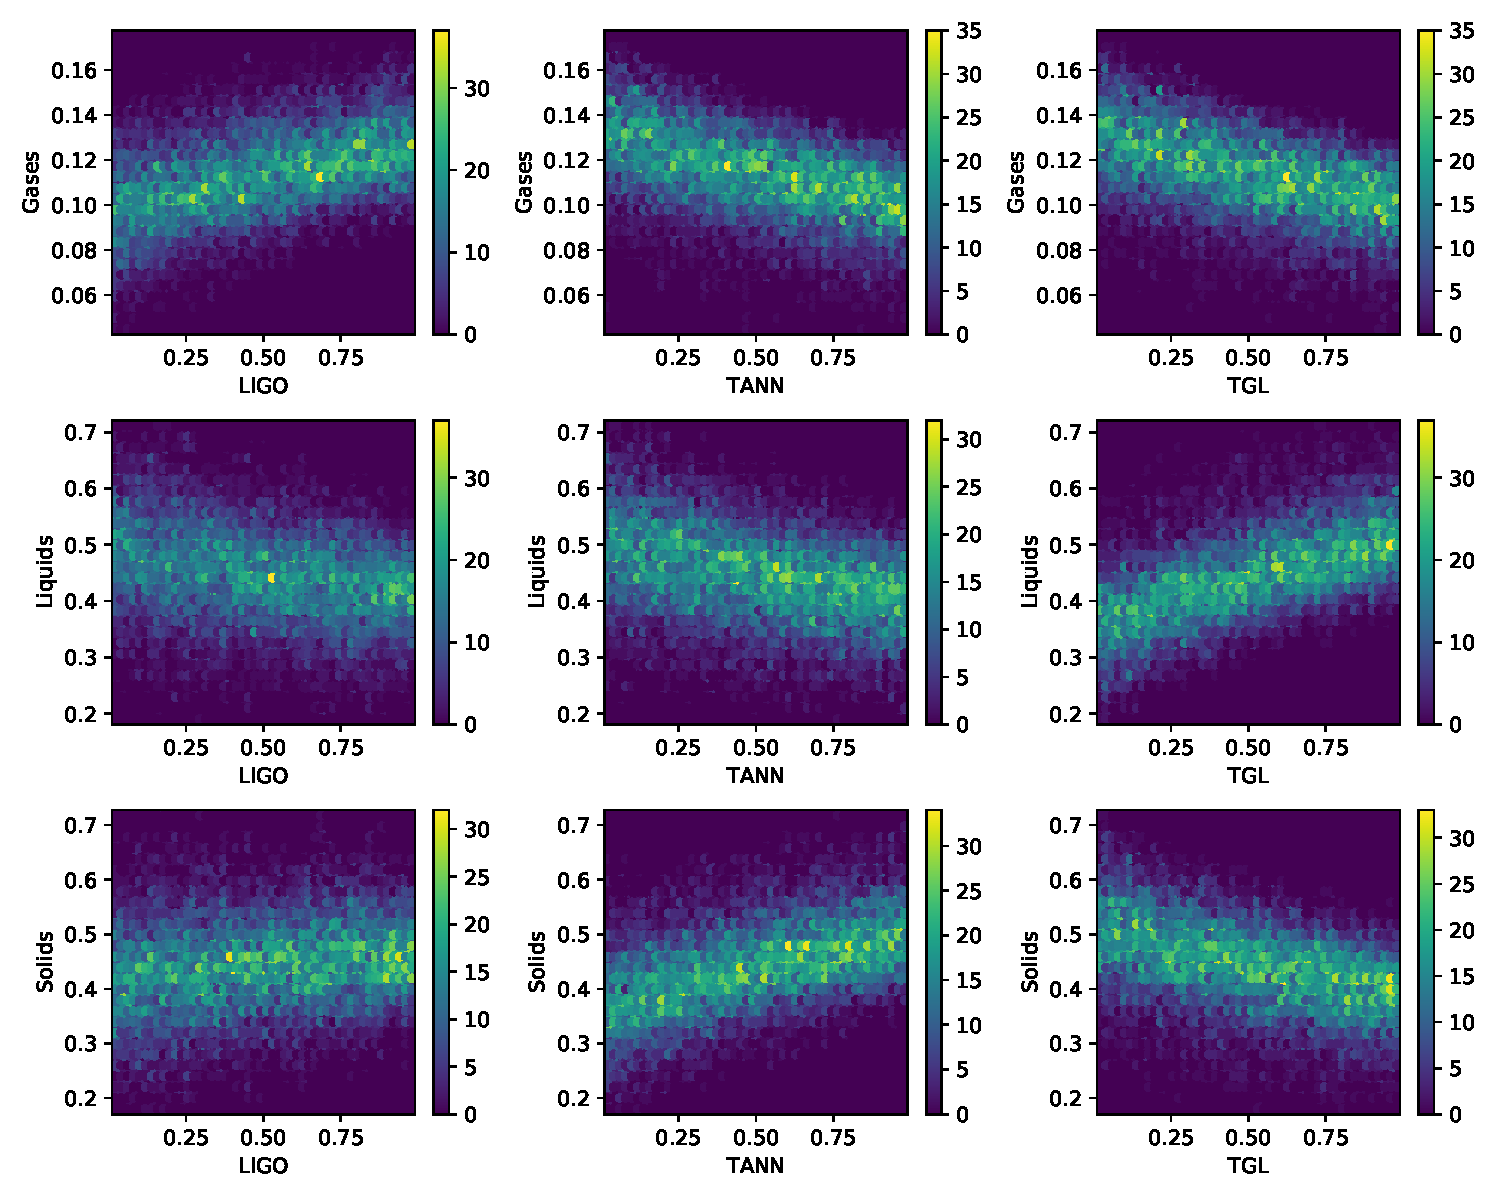
\includegraphics[width=\textwidth]{figures/sa-hexbin2-n1000.pdf}
    \caption{Batch reactor results for oxygen-rich lignin (LIGO), tannins (TANN), and triglycerides (TGL) using 16,000 samples. Reaction time is 10 seconds at 773.15 K and 101,325 Pa. Colorbar represents bin count.}
    \label{fig:batch-sa2}
\end{figure}

\begin{figure}[H]
    \centering
    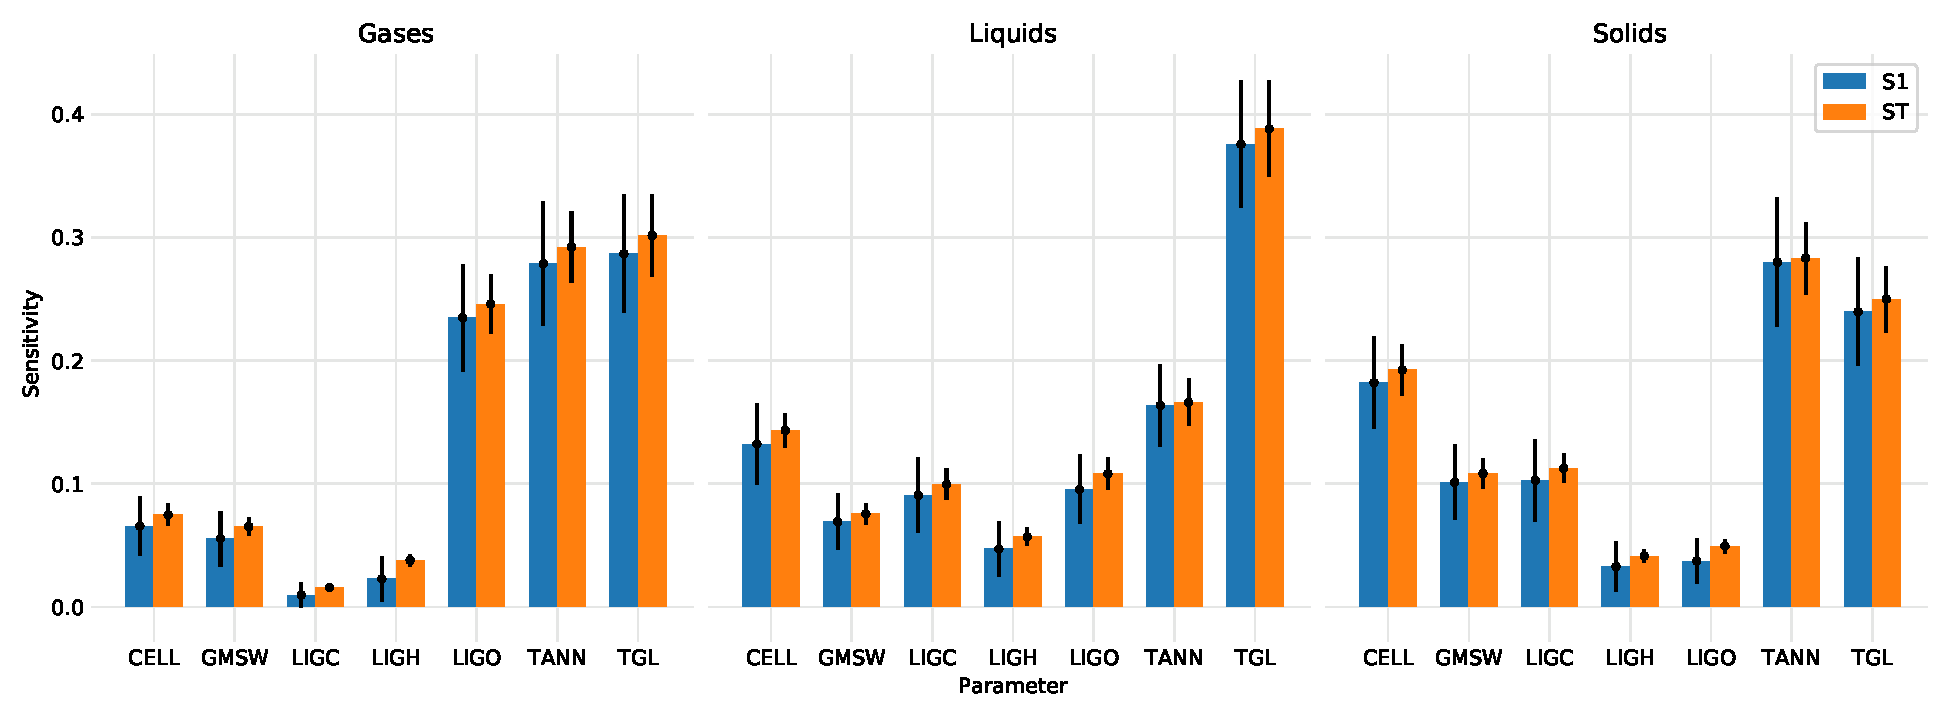
\includegraphics[width=\textwidth]{figures/sa-bar-n1000.pdf}
    \caption{First-order (S1) and total-order (ST) Sobol indices for biomass composition with reactants grouped as gases, liquids, and solids using 16,000 samples.}
    \label{fig:batch-sa3}
\end{figure}

\subsection{Blend3 biomass composition}

Several approaches were investigated to characterize the Blend3 feedstock data for use with the Debiagi pyrolysis kinetics. The characterization method discussed in the Debiagi et al. 2015 paper utilizes the carbon and hydrogen from ultimate analysis to determine the biomass composition \cite{Debiagi-2015}. To use this approach for the Blend3 feedstock, the mass fraction of C and H on a dry ash-free basis (last column in Table \ref{tab:blend3-ult-bases}) is used for the biomass characterization procedure.

\begin{table}[H]
    \centering
    \caption{Ultimate analysis bases for the Blend3 feedstock. Mass percent values are given for as-received (ar), dry, and dry ash-free (daf) basis.}
    \label{tab:blend3-ult-bases}
    \begin{tabular}{lrrrr}
        \toprule
        Element & \% ar & \% dry & \% daf & \% daf \\
        \midrule
        C        & 49.52 & 52.70 & 53.06 & 53.16 \\
        H        & 5.28  & 5.62  & 5.66  & 5.67  \\
        O        & 38.35 & 40.82 & 41.10 & 41.17 \\
        N        & 0.15  & 0.16  & 0.16  &       \\
        S        & 0.02  & 0.02  & 0.02  &       \\
        ash      & 0.64  & 0.68  &       &       \\
        moisture & 6.04  &       &       &       \\
        \bottomrule
    \end{tabular}
\end{table}

\textbf{Case 1:} The first approach to characterize the Blend3 feedstock was performed using a carbon mass fraction of 53.16\%, hydrogen mass fraction of 5.67\%, and splitting parameters $\alpha = 0.6$, $\beta = 0.8$, $\gamma = 0.8$, $\delta = 1.0$, and $\epsilon = 1.0$ which do not account for extractives in the feedstock. Results from this characterization are shown in Figure \ref{fig:blend3-biocharact-ult} and the associated biomass composition is given in Table \ref{tab:blend3-biocomp}. While this approach is useful for limited feedstock data, its accuracy is questionable when compared to experimental measurements. For example, chemical analysis of the Blend3 feedstock provides a lignin composition of 29.48\% (see Table \ref{tab:blend3-chem-analysis}) whereas the characterization method using ultimate analysis data estimates a total lignin composition greater than 59\%.

\begin{figure}[H]
    \centering
    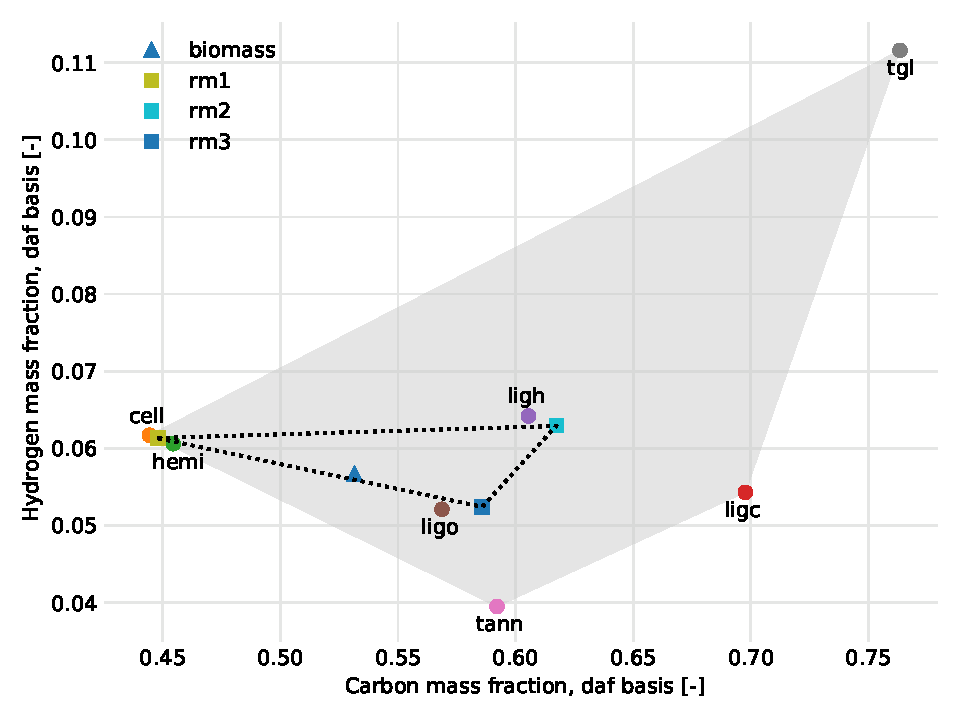
\includegraphics[width=0.8\textwidth]{figures/blend3-biocharact-ult.pdf}
    \caption{Characterization of the Blend3 feedstock using ultimate analysis data. Reference mixtures (rm) are labeled with square markers.}
    \label{fig:blend3-biocharact-ult}
\end{figure}

\textbf{Case 2:} To improve the Blend3 characterization based on ultimate analysis data, the splitting parameters were adjusted to account for extractives in the feedstock by using $\alpha = 0.56$, $\beta = 0.6$, $\gamma = 0.6$, $\delta = 0.78$, and $\epsilon = 0.88$. Also, since the uncertainty in the ultimate analysis data is unknown (see Table \ref{tab:blend3-ult}) the carbon mass fraction was adjusted to 51\% and the hydrogen mass fraction to 6\%. Results from these adjustments are presented in Figure \ref{fig:blend3-biocharact-ultmod} and Table \ref{tab:blend3-biocomp}.

\begin{figure}[H]
    \centering
    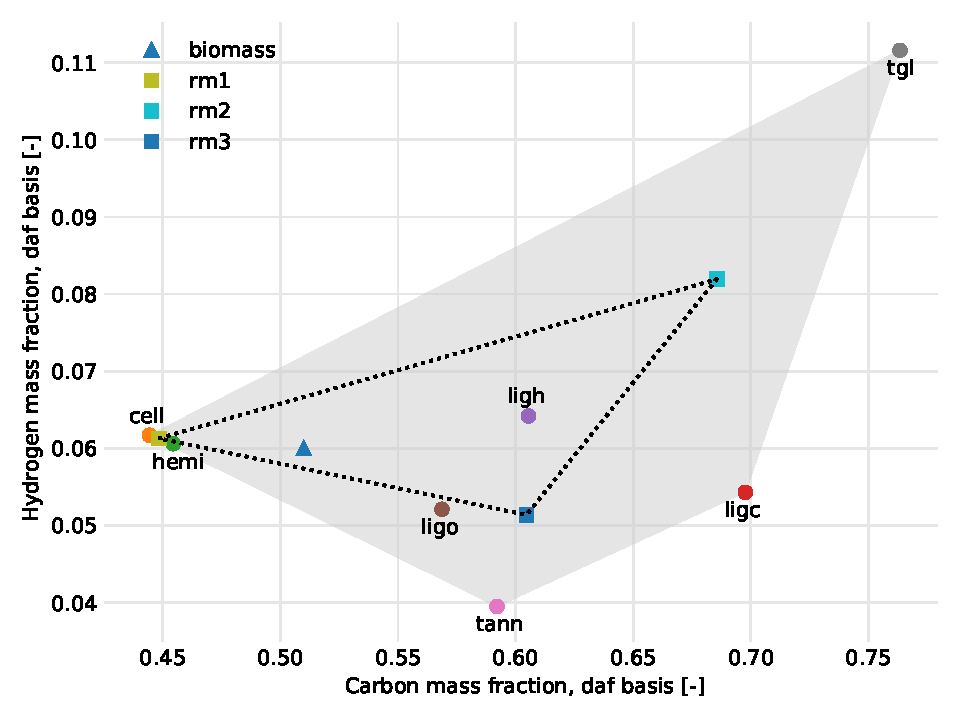
\includegraphics[width=0.8\textwidth]{figures/blend3-biocharact-ultmod.pdf}
    \caption{Characterization of the Blend3 feedstock using modified ultimate analysis data and adjusting the splitting parameters to account for extractives. Reference mixtures (rm) are labeled with square markers.}
    \label{fig:blend3-biocharact-ultmod}
\end{figure}

\textbf{Case 3:} The final approach to characterize the Blend3 feedstock, was to use chemical analysis data (see Table \ref{tab:blend3-chem-analysis}) to determine the biomass composition. As summarized in Table \ref{tab:biocomp-chem} the cellulose is represented by glucan while hemicellulose is comprised of xylan, mannan, galactan, arabinan, free fructose, free glucose, and sucrose. The measurement technique to determine the lignin components is unknown; therefore, the lignin is evenly divided into the carbon, hydrogen, and oxygen-rich fractions. Tannins are represented by acetyl, water extractives, and ethanol extractives while ash is the non-structural and structural inorganics. Triglycerides were not present in the Blend3 feedstock. Finally, the biomass composition based on the chemical analysis measurements is given in Table \ref{tab:blend3-biocomp}.

\begin{table}[H]
    \centering
    \caption{Biomass composition represented by chemical analysis components.}
    \label{tab:biocomp-chem}
    \begin{tabular}{lp{3in}}
        \toprule
        Biomass composition & Chemical analysis data \\
        \midrule
        cellulose     & glucan \\
        \addlinespace[0.1in]
        hemicullulose & xylan, mannan, galactan, arabinan, free fructose, free glucose, sucrose \\
        \addlinespace[0.1in]
        lignin-c      & lignin / 3 \\
        \addlinespace[0.1in]
        lignin-h      & lignin / 3 \\
        \addlinespace[0.1in]
        lignin-o      & lignin / 3 \\
        \addlinespace[0.1in]
        tannins       & acetyl, water extractives, ethanol extractives \\
        \addlinespace[0.1in]
        triglycerides & not applicable \\
        \addlinespace[0.1in]
        ash           & non-structural inorganics, structural inorganics \\
        \bottomrule
    \end{tabular}
\end{table}

\begin{table}[H]
    \centering
    \caption{Biomass composition for the Blend3 feedstock. Values are reported as mass percent on a dry ash-free basis (\% daf).}
    \label{tab:blend3-biocomp}
    \begin{tabular}{lrrr}
        \toprule
        Biomass composition & Case 1 & Case 2 & Case 3 \\
        \midrule
        cellulose     & 26.38 & 39.24 & 39.19 \\
        hemicellulose & 14.33 & 25.12 & 23.26 \\
        lignin-c      & 7.84  & 8.57  & 9.89  \\
        lignin-h      & 5.27  & 3.11  & 9.89  \\
        lignin-o      & 46.18 & 18.00 & 9.89  \\
        tannins       & 0.00  & 2.95  & 7.88  \\
        triglycerides & 0.00  & 3.01  & 0.00  \\
        \bottomrule
    \end{tabular}
\end{table}

\subsection{Blend3 batch reactor conversion and yields}

The final concentrations in the batch reactor after 10 seconds of reaction at 500$^{\circ}$C are shown in Table \ref{tab:blend3-batch-final}. These results do not utilize the thermo data for the Debiagi kinetics; therefore, they neglect exothermic or endothermic effects from heats of reactions. As the table shows, concentrations vary considerably based on the initial biomass composition. Therefore, it is essential to correctly characterize the biomass composition to obtain reasonable results from the Debiagi pyrolysis kinetics.

\begin{table}[H]
    \centering
    \caption{Final batch reactor concentrations for Blend3 feedstock (no thermo). Biomass composition based on ultimate analysis (Case 1), modified ultimate analysis and splitting parameters (Case 2), and chemical analysis (Case 3).}
    \label{tab:blend3-batch-final}
    \begin{tabular}{lrrr}
        \toprule
        Final concentration (\% mass) & Case 1 & Case 2 & Case 3 \\
        \midrule
        gases         & 18.40 & 15.93 & 14.99 \\
        liquids       & 40.08 & 55.79 & 52.51 \\
        solids        & 20.84 & 16.25 & 20.92 \\
        metaplastics  & 20.68 & 12.04 & 11.59 \\
        \bottomrule
    \end{tabular}
\end{table}

For the Blend3 biomass composition based on the chemical analysis data (Case 3), evolutions of the gas, liquid, solid, and metaplastic species are shown in Figures \ref{fig:blend3-case3-gases-liquids} and \ref{fig:blend3-case3-solids-meta}. A comparison of the total gas, liquid, solid, and metaplastic species is given in Figure \ref{fig:blend3-case3-phases-temp} along with the batch reactor temperature profile. Figure \ref{fig:blend3-case3-final} depicts the final concentrations of the chemical species at 10 seconds of reaction time. At 500$^{\circ}$C the metaplastic species remain in the reactor and contribute to the total solids concentration.

\begin{figure}[H]
    \makebox[\textwidth][c]{
        \begin{subfigure}{1.4\textwidth}
            \centering
            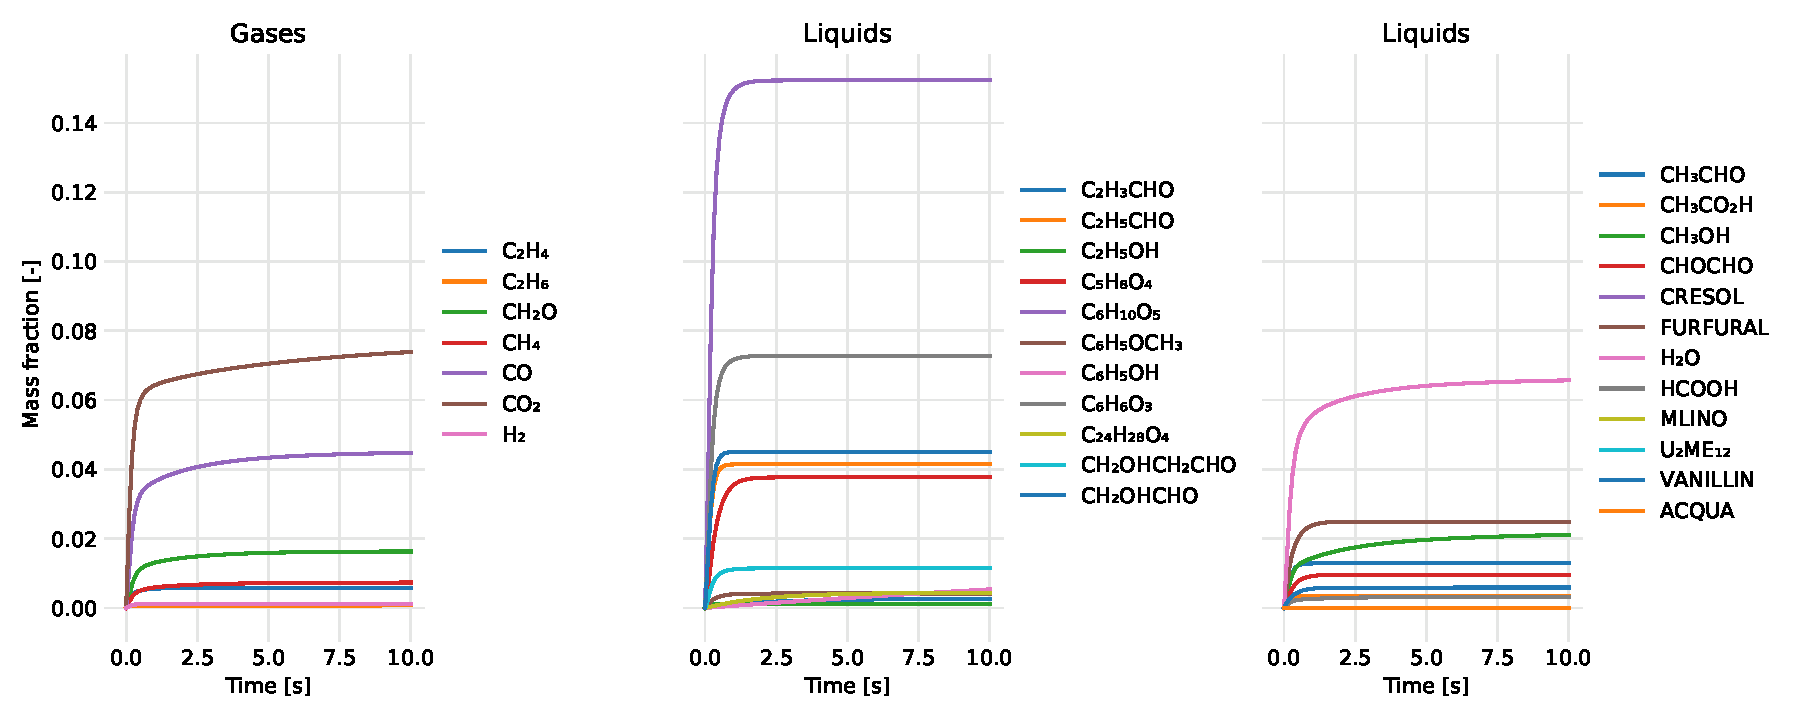
\includegraphics[width=\textwidth]{figures/blend3-case3-gases-liquids.pdf}
            \caption{Without thermodynamics.}
        \end{subfigure}
    }
    \makebox[\textwidth][c]{
        \begin{subfigure}{1.4\textwidth}
            \centering
            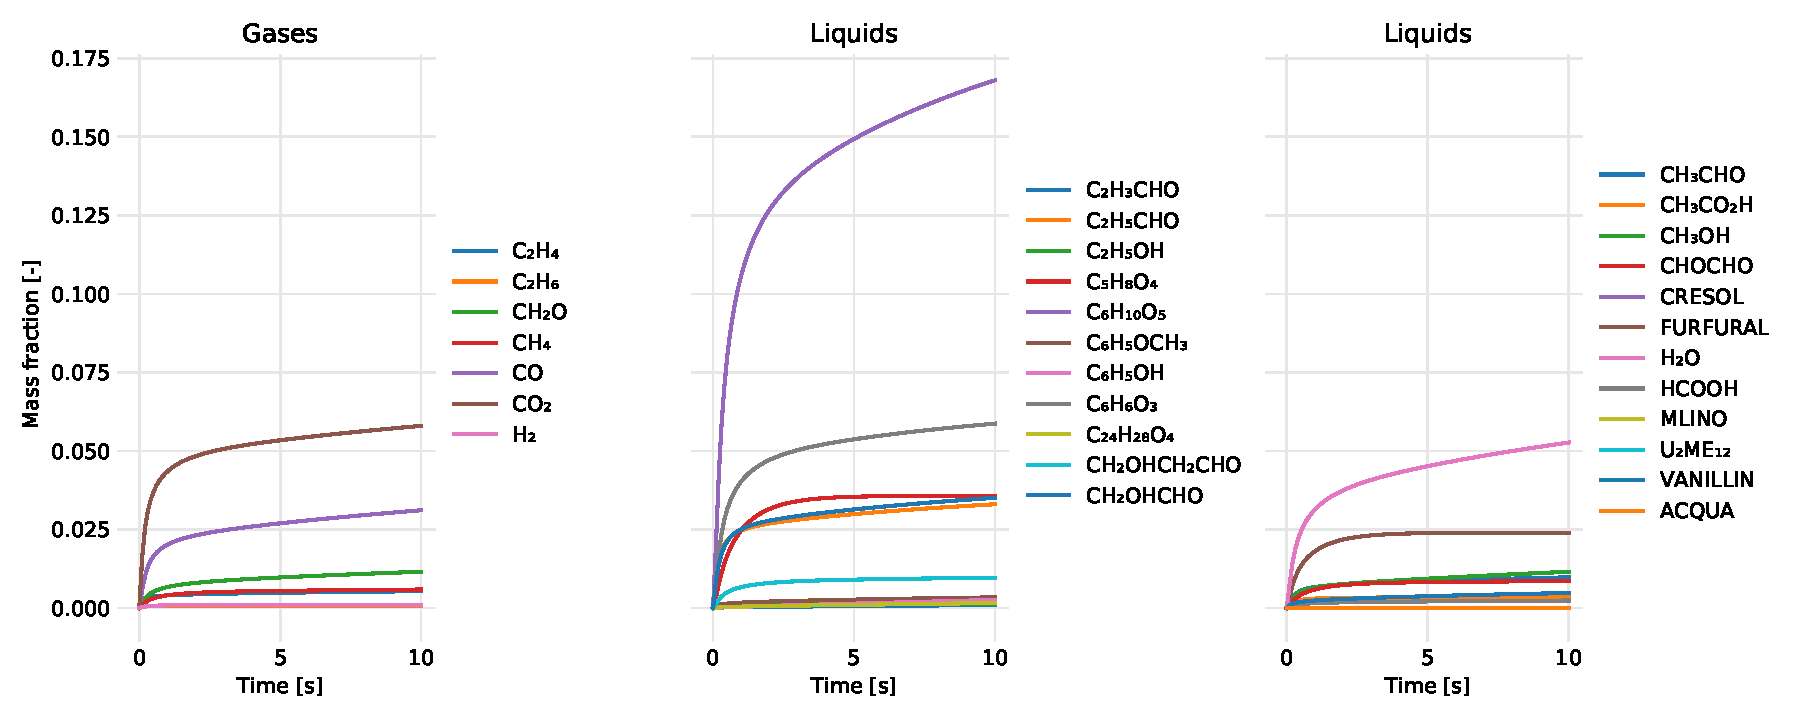
\includegraphics[width=\textwidth]{figures/blend3-case3-gases-liquids-thermo.pdf}
            \caption{With thermodynamics.}
        \end{subfigure}
    }
    \caption{Batch reactor gas and liquid concentrations for Blend3 feedstock based on Case 3 biomass composition.}
    \label{fig:blend3-case3-gases-liquids}
\end{figure}

\begin{figure}[H]
    \begin{subfigure}{\textwidth}
        \centering
        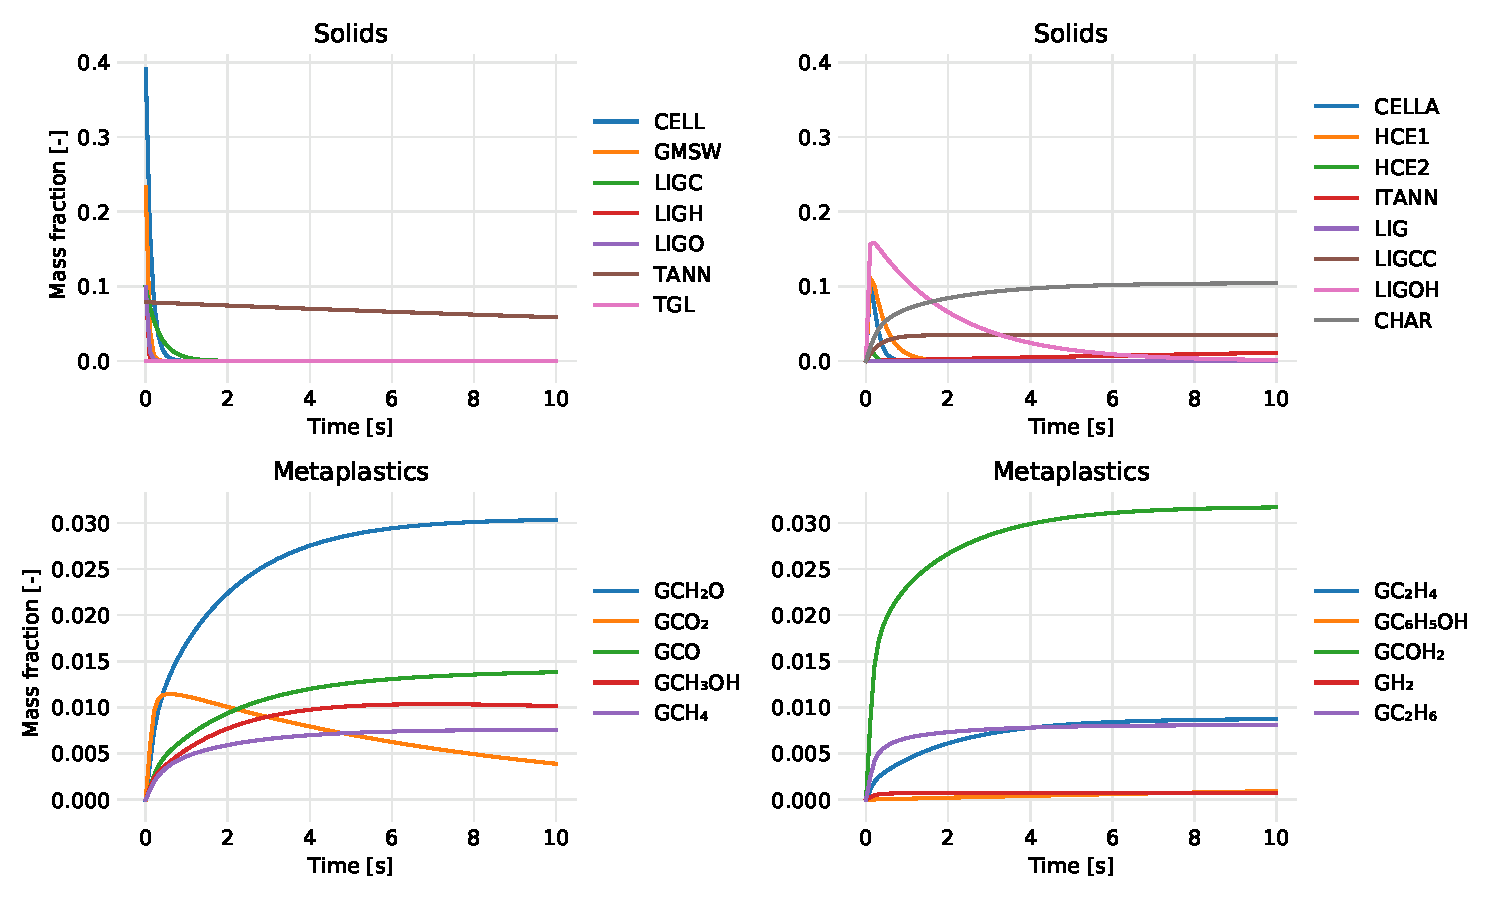
\includegraphics[width=\textwidth]{figures/blend3-case3-solids-meta.pdf}
        \caption{Without thermodynamics.}
    \end{subfigure}
    \begin{subfigure}{\textwidth}
        \centering
        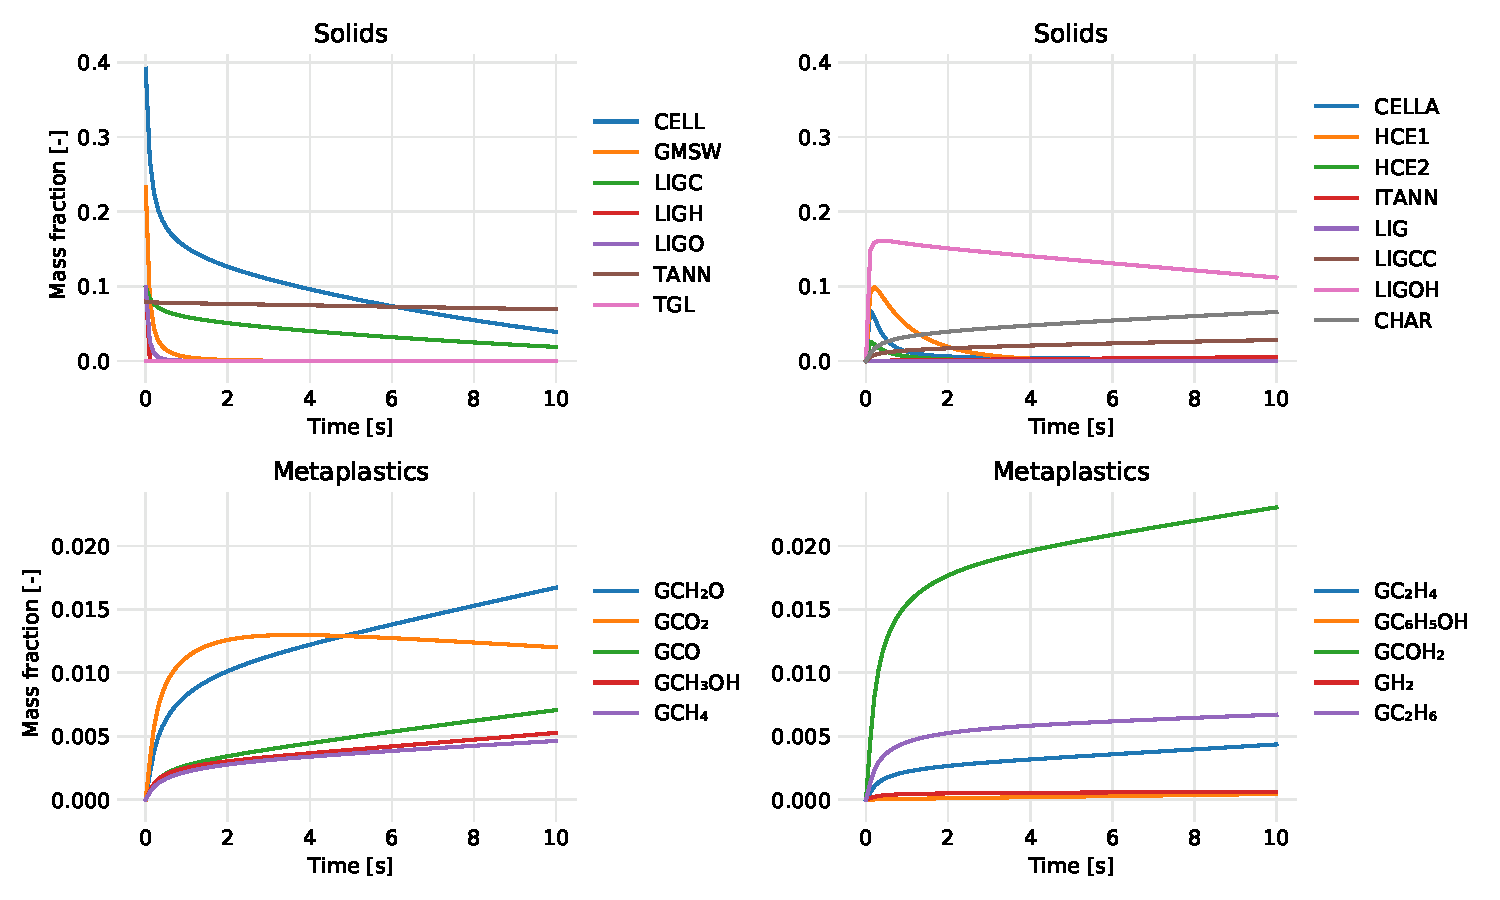
\includegraphics[width=\textwidth]{figures/blend3-case3-solids-meta-thermo.pdf}
        \caption{With thermodynamics.}
    \end{subfigure}
    \caption{Batch reactor solid and metaplastic concentrations for Blend3 feedstock based on Case 3 biomass composition.}
    \label{fig:blend3-case3-solids-meta}
\end{figure}

\begin{figure}[H]
    \begin{subfigure}{\textwidth}
        \centering
    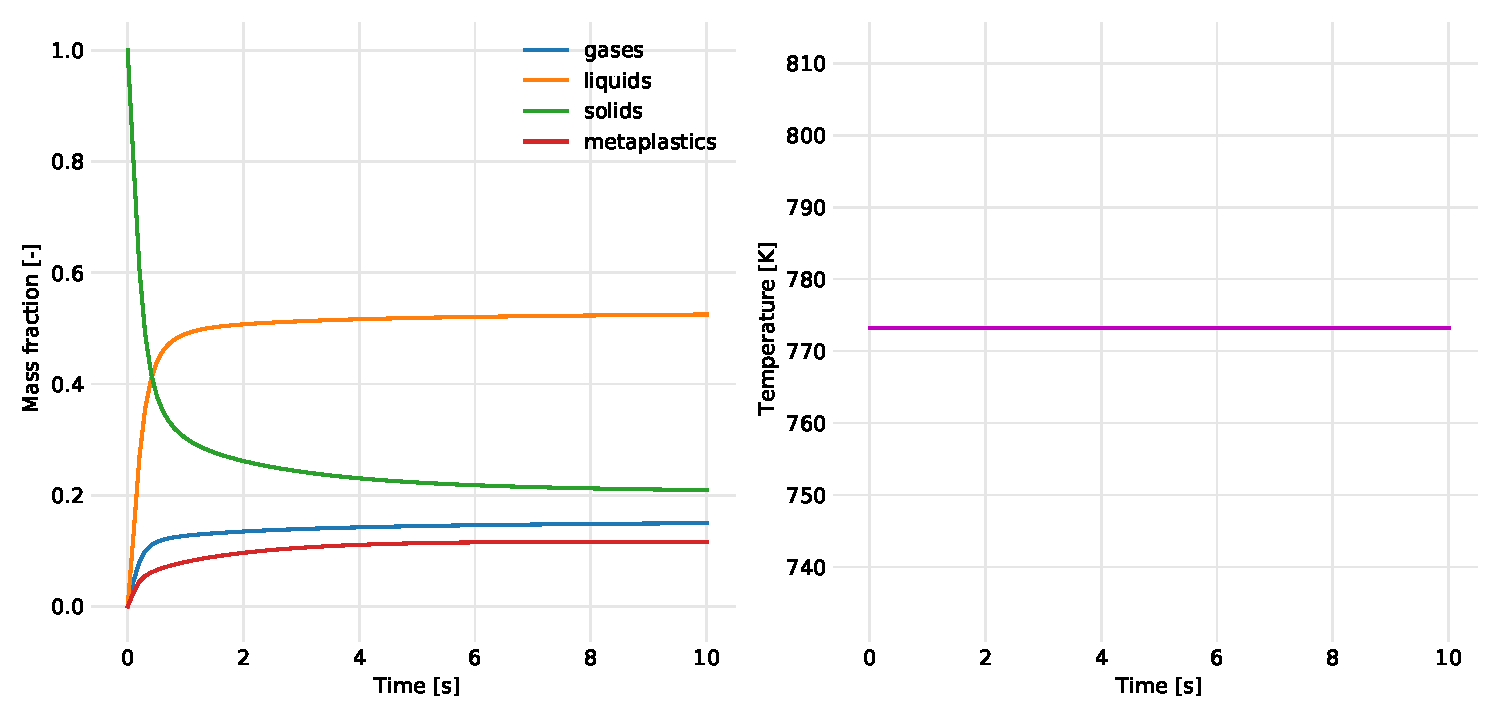
\includegraphics[width=\textwidth]{figures/blend3-case3-phases-temp.pdf}
        \caption{Without thermodynamics.}
    \end{subfigure}
    \begin{subfigure}{\textwidth}
        \centering
    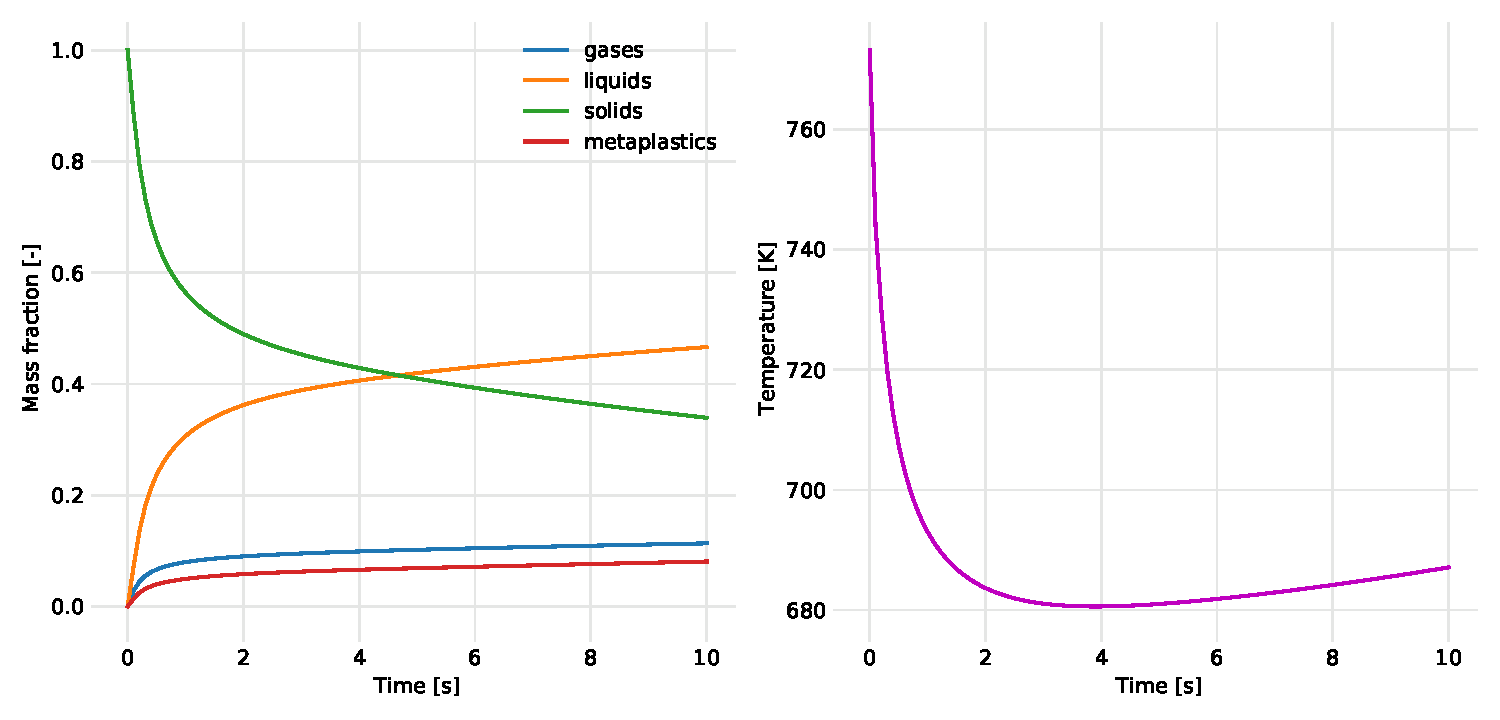
\includegraphics[width=\textwidth]{figures/blend3-case3-phases-temp-thermo.pdf}
        \caption{With thermodynamics.}
    \end{subfigure}
    \caption{Comparison of the gas, liquid, solid, and metaplastic phases in the batch reactor for the Blend3 feedstock based on Case 3 biomass composition. Reactor temperature during the reaction process.}
    \label{fig:blend3-case3-phases-temp}
\end{figure}

\begin{figure}[H]
    \makebox[\textwidth][c]{
        \begin{subfigure}{1.3\textwidth}
            \centering
            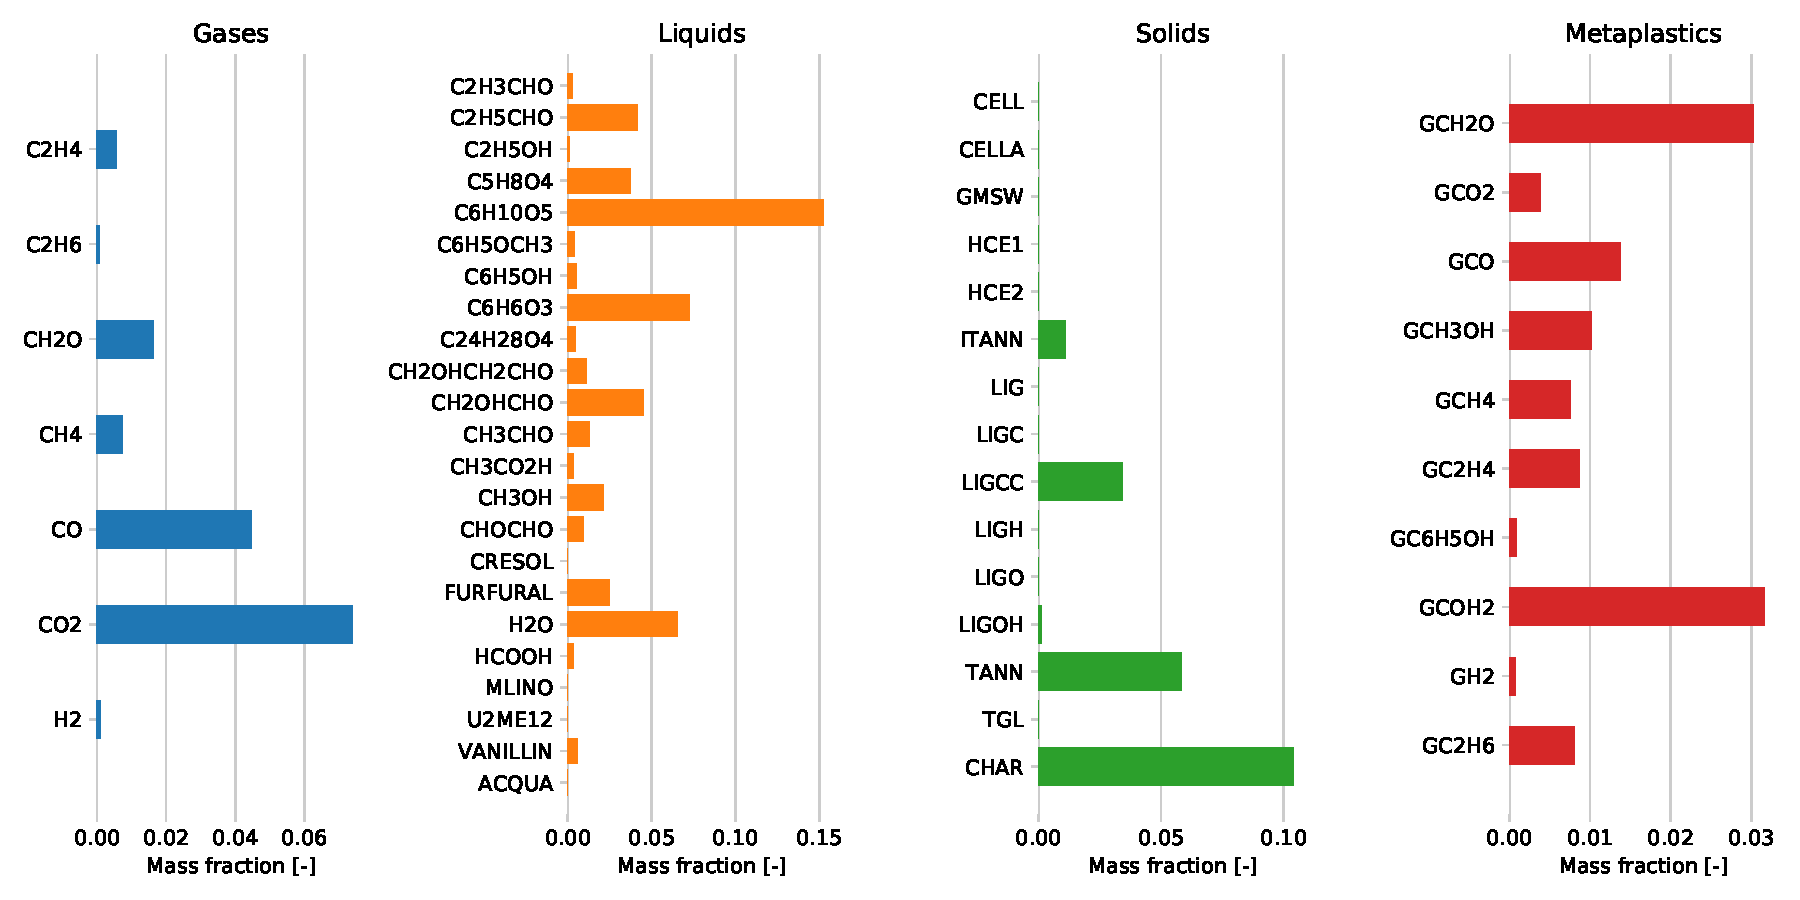
\includegraphics[width=\textwidth]{figures/blend3-case3-final.pdf}
            \caption{Without thermodynamics.}
        \end{subfigure}
    }
    \makebox[\textwidth][c]{
        \begin{subfigure}{1.3\textwidth}
            \centering
            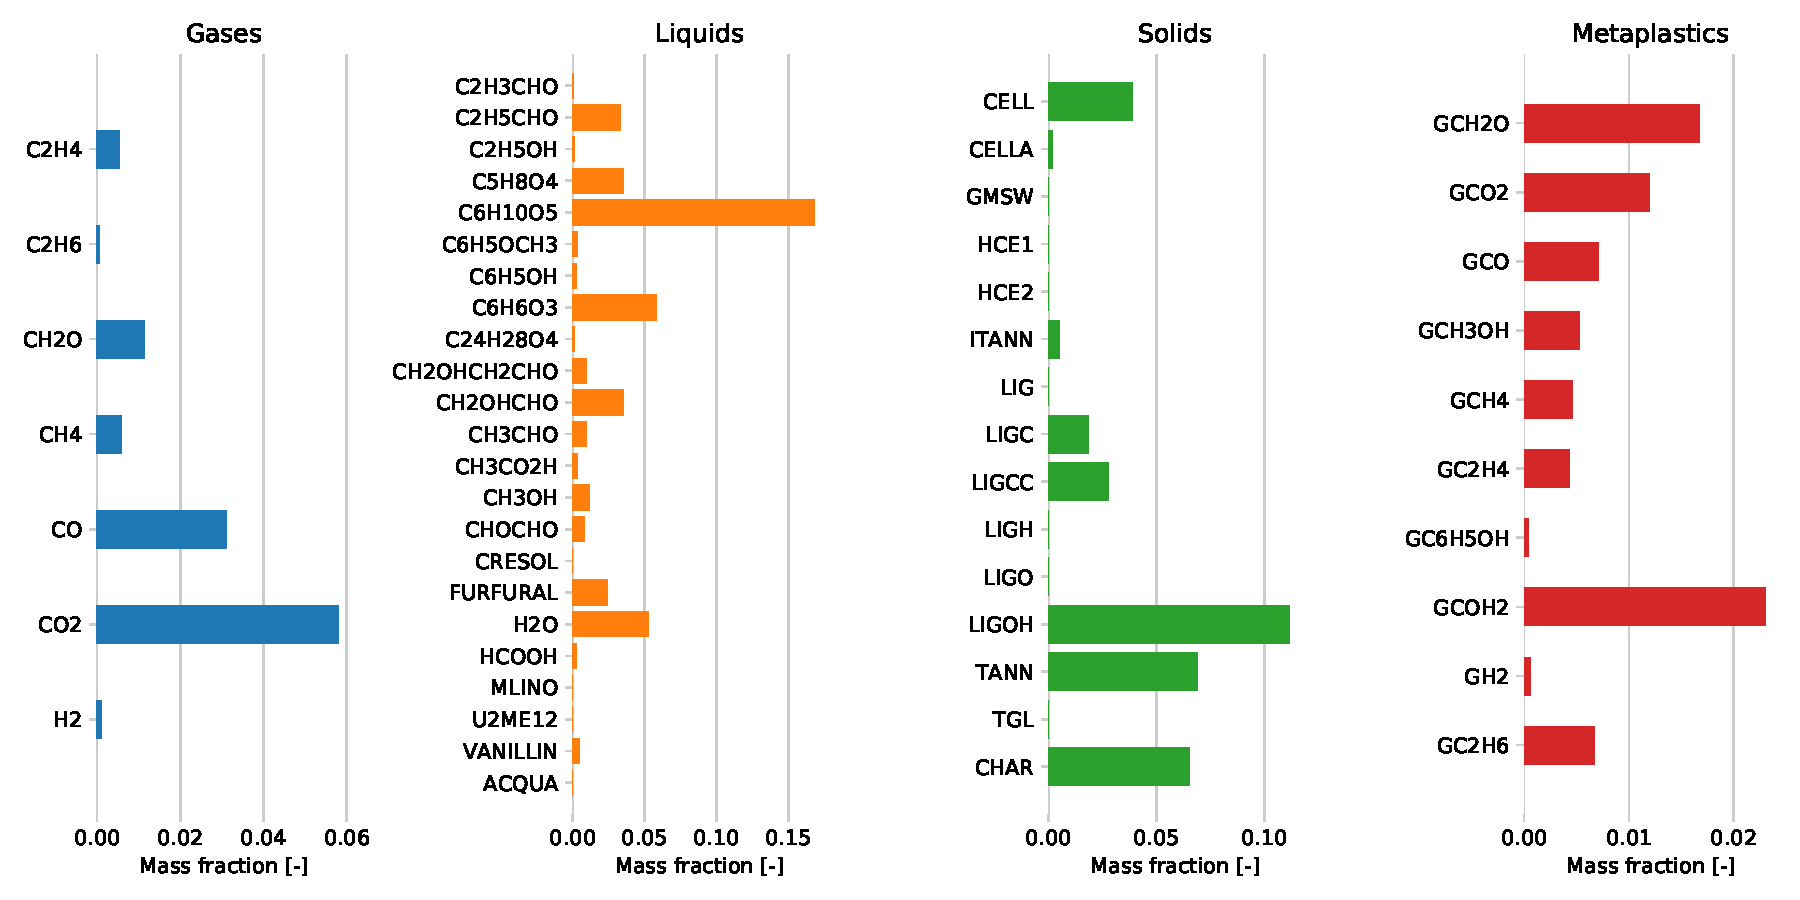
\includegraphics[width=\textwidth]{figures/blend3-case3-final-thermo.pdf}
            \caption{With thermodynamics.}
        \end{subfigure}
    }
    \caption{Final batch reactor concentrations for Blend3 feedstock based on Case 3 biomass composition.}
    \label{fig:blend3-case3-final}
\end{figure}

\subsection{Blend3 entrained flow reactor model}

Here.
